Es gibt wenige große Denker, die sich mit der Bibliothek als Idee
beschäftigt haben. Die meisten unter ihnen wie Leibniz, Lessing oder
Goethe waren selber Bibliothekare und deshalb eher mit praktischen
Dingen beschäftigt oder von ihr geblendet (wie Borges). Es scheint als
wäre sie ein solches Faszinosum, dass sie, wie bei der Heisenbergschen
Unschärferelation, weder an ihrem Ort noch an ihrer Aktivität (das heißt
Bewegung) dingfest gemacht werden kann. Zu den wenigen \enquote{Großen},
die sich substantiell zum Phänomen Bibliothek geäußert haben, gehören
Michel Foucault zur Bibliothek als Ort und Bruno Latour zum
\enquote{Akteur-Netzwerk} des Sammelns. Diese beiden Perspektiven sollen
im Folgenden zusammengeführt werden.

Lange Zeit war die Normbeschreibung der Bibliothek die einer
\enquote{speziellen Informationseinrichtung},\footnote{Kaegbein, Paul
  (1973): Bibliotheken als spezielle Informationssysteme. In:
  Zeitschrift für Bibliothekswesen und Bibliographie 20, S. 425--442. --
  kritisch dazu: Jochum, Uwe (2011): Die Selbstabschaffung der
  Bibliothek. In: Uwe Jochum und Armin Schlechter (Hg.): Das Ende der
  Bibliothek? Vom Wert des Analogen. 1. Aufl. Frankfurt am Main:
  Klostermann, S. 11--25.} ohne dass hinterfragt wurde, ob diese
Verortung ihr gut tut. In den letzten Jahren hat jedoch nicht nur die
Informationswissenschaft, auf die sich ja die Bibliothekswissenschaft
lange Zeit als Mutterdisziplin bezog, eine kopernikanische Wende
vollzogen: Vom IT-lastigen Systemparadigma zum sozio-kognitiven Ansatz
und zur Anerkennung der Komplexität des Informationsverhaltens realer
Nutzer mit Körper und in einem sozialen Kontext.\footnote{Ingwersen,
  Peter; Järvelin, Kalervo (2005): The turn: integration of information
  seeking and retrieval in context. Dordrecht u.a.: Springer (Kluwer
  international series on information retrieval). -- Day, Ronald E.
  (2014): Indexing it all. The subject in the age of documentation,
  information, and data. Boston: MIT Press.} Eine solche Wende scheint
sich in der Sicht auf Bibliotheken nicht nur aufzudrängen, sondern auch
durchzusetzen. Einer der ersten, der eindringlich auf die blinden Flecke
der Bibliothekswissenschaft hingewiesen hat, war Wayne Wiegand in einem
oft referenzierten Artikel in \emph{Library Quarterly}.\footnote{Wiegand,
  Wayne A. (1999): Tunnel Vision and Blind Spots. What the Past Tells Us
  about the Present; Reflections on the Twentieth-Century History of
  American Librarianship. In: Library Quarterly 69, S. 1--32. - vgl.
  Hobohm, Hans-Christoph (2005): Desiderate und Felder
  bibliothekswissenschaftlicher Forschung. In: Petra Hauke
  (Hg.):Bibliothekswissenschaft quo vadis? = Library Science quo vadis?
  Eine Disziplin zwischen Traditionen und Visionen; Programme Modelle
  Forschungsaufgaben. München: Saur, S. 47--64. -- sowie: Hobohm,
  Hans-Christoph (2007): Bibliothek(swissenschaft) 2.0. Neue Auflage
  oder Wende in Forschung und Lehre? In: LIBREAS (10/11).} Er wies in
Zeiten der Umbenennung der Library Schools in die späteren iSchools
darauf hin, dass wir dem komplexen Phänomen Bibliothek mit dem
IT-System-Paradigma nicht gerecht werden. Seine Analyse war, dass wir
zwei blinde Flecke im Blick auf Bibliotheken haben: Wir kümmer(te)n uns
zu wenig um den Ort des Nutzerkontaktes, und wir können nicht
einschätzen, was das ist, was die meisten Nutzer in Bibliotheken machen:
Nämlich Lesen.

Der Ort ist mittlerweile stark ins Zentrum der
bibliothekswissenschaftlichen Argumentation gerückt. Bibliothek als
\enquote{Dritter Ort} ist fast schon ein Gemeinplatz. Immer noch nicht
im Blick ist das, was die Nutzer eigentlich in der Bibliothek machen.
Das öffnet natürlich auch Türen für Experimente wie Makerspaces, bei
denen man merkt, dass auch mit solchen Aktivitäten in Bibliotheken die
\enquote{richtigen} Dinge passieren und das sie dem \enquote{Phänomen
Bibliothek} irgendwie gerecht werden.\footnote{Koh, Kyungwon (2013):
  Adolescents' information-creating behavior embedded in digital Media
  practice using scratch. In: Journal of the American Society for
  Information Science and Technology 64 (9), S. 1826--1841. DOI:
  10.1002/asi.22878.}

Aus verschiedenen Diskursen\footnote{Hobohm, Hans-Christoph (2013):
  Bibliothek im Wandel. In: Rainer Kuhlen, Wolfgang Semar und Dietmar
  Strauch (Hg.): Grundlagen der praktischen Information und
  Dokumentation. 6. Aufl. Berlin: De Gruyter Saur, S. 622--632.} kann
man unabhängig vom Informationsparadigma folgende Grundfunktionen für
Bibliotheken postulieren. Sie sind:

\begin{itemize}
\item
  Kultisch-herrschaftlicher, hegemonialer Knoten im Netz der
  Machtstruktur
\item
  Instanz für das kulturelle Gedächtnis (=Funktionsgedächtnis)
\item
  Werkstatt / Instrument zur Beförderung menschlicher Erkenntnis.
\end{itemize}

Der aktuelle Beleg für die erste Funktion kommt Mitte der 1990er Jahre
aus Dänemark, wo Jens Thorhauge im Auftrag der EU das berühmte
Whitepaper zu \enquote{Bibliotheken in der Informationsgesellschaft}
verfasst hatte.\footnote{Thorhauge, Jens et al (1996): Public Libraries
  and the Information Society. Study on behalf of the European
  Commission, DG-XIII/E/4, Prolib/PLIS 10340. Brüssel: EU, S. 3.} Neben
der (aktiven!) Hegemonialfunktion der Bibliothek in der Demokratie wird
aber schon außerordentlich stark der Ort der Bibliothek betont, wenn sie
als \enquote{Hauptakteur bei der lokalen Implementation der
Informationsgesellschaft} bezeichnet wird und ihr folgende Aufgaben
zugeschrieben werden:

\begin{itemize}
\item
  Partner für Demokratie und Informationsfreiheit
\item
  Ort für Bildung und Lernen; Lieferant des Rohstoffes für Wissen
\item
  Informationstechnikzentrum
\item
  Kultureller Ort: \enquote{\emph{a good social spot}}
\end{itemize}

15 Jahre später kommt wieder aus Dänemark die genauere Beschreibung für
Ort und Raum der Bibliothek und ihrer Funktion bei der Stadtentwicklung:
Das \enquote{Four Spaces Model}\footnote{Hvenegaard, Casper; Jochumsen,
  Henrik; Skot-Hansen, Dorte (2011): Biblioteket i byudviklingen.
  Oplevelse, kreativitet og innovation. Kopenhagen: Danmarks
  Biblioteksforening; Det Informationsvidenskabelige Akademi. --
  Jochumsen, Henrik; Hvenegaard Rasmussen, Casper (2012): The four
  spaces. A new model for the public library. In: New Library World 112
  (11/12), S. 586--597. -- Skot-Hansen, Dorte; Hvenegaard Rasmussen,
  Casper; Jochumsen, Henrik (2013): The role of public libraries in
  culture-led urban regeneration. In: New Library World 114 (1), S.
  7--19. -- Jochumsen, Henrik; Skot-Hansen, Dorte; Hvenegaard Rasmussen,
  Casper (2014): Erlebnis, Empowerment, Beteiligung und Innovation: Die
  neue Öffentliche Bibliothek. In: Olaf Eigenbrodt und Richard Stang
  (Hg.): Formierungen von Wissensräumen. Optionen des Zugangs zu
  Information und Bildung. Berlin: De Gruyter Saur (Age of access? --
  Grundfragen der Informationsgesellschaft, 3), S. 67--80.} der
Kopenhagener Informationswissenschaftler Hvenegaard, Jochumsen und
Skot-Hansen, die die vier Räume der Öffentlichen Bibliothek so
beschreiben:

\begin{itemize}
\item
  Inspirationsraum
\item
  Lernraum
\item
  Treffpunkt
\item
  Performativer Raum\footnote{op. cit 2014, 70 (ursprünglich 2012)}
\end{itemize}

und die Bibliothek in ihrer Rolle in der Stadtentwicklung gleichzeitig
als

\begin{itemize}
\item
  Place (Icon, Placemaker, Catalyst)
\item
  Space (open minded meeting place, public domain, experience-space)
\item
  Relationship (partnership and creative alliances, hybrid cultural
  arenas, creative entrepreneurs)\footnote{op cit. 2011, 16 (Übersetzung
    ins Englische Knud Schulz)}
\end{itemize}

kennzeichnen.

Dass Bibliotheken mittlerweile ikonische Qualität im Stadtbild, aber
auch auf einem Wissenschafts-Campus haben, bezeugen Beispiele wie die
\enquote{Wissenspyramide} in Ulm, die Public Libraries in Seattle oder
in Birmingham bzw. der Konus der TU Delft, die Amöbe der BTU Cottbus
oder \enquote{The Brain} der FU Berlin. Die Inszenierung der Bibliothek
als Erfahrungsraum hat schon eine lange Tradition. Nicht nur
traditionelle Lesesäle, sondern auch neue Angebote und Funktionen wie
Cafés, Restaurants, \enquote{Salons} oder hyperaktive Musikbibliotheken
wie \enquote{Kirjasto 10} in Helsinki, Multimedia Experimentierflächen
wie in Dokk1 -- im \enquote{Urban Media Space} -- in Aarhus oder wie bei
vielen Makerspaces nicht nur in Stadtbibliotheken zeugen davon.

\begin{figure}[htbp]
\centering
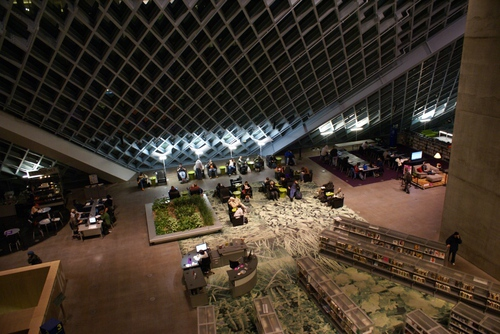
\includegraphics{img/hobohm-1.jpg}
\caption{Abbildung 1: Seattle Public Library (2014)}
\end{figure}

An dieser Stelle kann man einen der wenigen großen Denker, die die
Bibliothek thematisiert haben, erwähnen. Michel Foucault\footnote{Foucault,
  Michel (2005): Die Heterotopien. Zwei Radiovorträge ; {[}7. und 21.
  Dezember 1966{]}. Frankfurt am Main: Suhrkamp (Zweisprachige Ausg.),
  S. 46.} ordnet sie explizit den Heterotopien zu, den anderen Räumen,
die eben nicht utopisch sind, aber doch anders, anderswo, divers oder
herausgehoben. Interessanterweise ist einer der \enquote{fünf
Grundsätze}, die Foucault Heterotopien zuschreibt, auch der der
Hetero\emph{chronie}, das heißt es sind die Heterotopien, die einerseits
mit der Zeit brechen, aber auch Zeitspeicher darstellen.\footnote{Chlada,
  Marvin (2005): Heterotopie und Erfahrung. Abriss der Heterotopologie
  nach Michel Foucault. Aschaffenburg: Alibri. S. 91.} Gerne vergisst
man die Zeit beim Stöbern in Bibliotheksbeständen und trifft auf den
Speicher des aus der Zeit herausgehobenen kulturellen Erbes. Wir werden
auf dieses Verhältnis von Ort und Zeit noch einmal zu sprechen kommen.

Der Ort (Place) bleibt nicht nur der zweidimensionale, flache Punkt auf
der Karte, sondern erhält sowohl eine symbolische Erhöhung als auch
aktive Funktionen als \enquote{Maker} und Katalysator. Schon hier
erscheint die Bibliothek als besonderer (beziehungsweise besonders
ruhiger) Akteur: Ein Katalysator ist ein Stoff, der allein durch seine
Anwesenheit Reaktionen beschleunigt oder überhaupt erst ermöglicht,
\enquote{ohne verbraucht zu werden}.\footnote{Wikipedia:
  \url{https://de.wikipedia.org/wiki/Katalysator}, 12.9.2015.} Die
vielen Diskussionen um die ökonomische Wirksamkeit von Bibliotheken und
ihres \enquote{Return of Investment} (ROI) könnten diesem entsprechen.
Aber auch die Nutzung von Bibliotheken tatsächlich als städtebauliche
oder institutionelle Ikone deutet auf das Wirken genau dieser Funktion,
ohne dass sich die Urheber entsprechender Bauten beziehungsweise die
Verwender von deren Abbildungen auf Werbemedien\footnote{Wenn zum
  Beispiel die FU Berlin oder das Land Brandenburg mit ihren ikonischen
  Bibliotheksbauten Imagebildung betreiben (Phililogikum Norman Foster
  Bau \enquote{The Brain}; IKMZ der BTU Cottbus, Herzog \& de Meuron).}
dessen bewusst wären.

\begin{figure}[htbp]
\centering
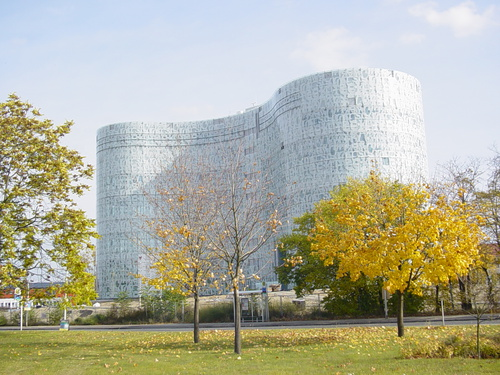
\includegraphics{img/hobohm-2.jpg}
\caption{Abbildung 2: Hochschulbibliothek der BTU Cottbus (2006)}
\end{figure}

Es gibt eine ganze Reihe von Ideen zu besonderen beziehungsweise
\enquote{dritten Orten}: von den \emph{lieux anthropologiques} (im
Gegensatz zu den \emph{lieux de passage}) bei Marc Augé, dem
\enquote{\emph{Third Place}} zwischen privat und öffentlich/beruflich
bei Ray Oldenbourg, den hybriden Räumen (nicht fremd/nicht Heimat) bei
Homi Bhabha oder dem \enquote{\emph{Third Space}} von Edward Soja, alle
weisen ähnliche Charakteristika auf, wie wir sie bei Bibliotheken
finden: Sie werden als neutral (politisch ungebunden), nivellierend
(jeder ist willkommen), kommunikativ (Konversation = Hauptaktivität),
niedrigschwellig (offene Strukturen), regelmäßig (Stammgäste,
\enquote{Kundenbindung}), niedrig profiliert (keine kommerziellen
Marken, kein Branding), als spielerisch (Atmosphäre, \enquote{ohne
endgültiges Ergebnis}) oder als \enquote{aushäusig} (weg von zu Hause)
beschrieben. Ort und Raum (Place und Space) lassen sich nicht
trennscharf auseinander halten, worauf zum Beispiel auch die Rede vom
Raum als dritten Pädagogen hindeutet.\footnote{Malaguzzi, Loris; Ceppi,
  Giulio; Zini, Michele (1998): Children, spaces, relations. Metaproject
  for an environment for young children. Reggio Emilia, Italy: Reggio
  Children. (Malaguzzi wird der Begriff in den 1970er Jahren
  zugeschrieben. Interessant aber auch, dass er hier in diesem neueren
  Buch von \enquote{relational space} spricht.)} Wenn sich Bibliotheken
zunehmend als Einrichtungen der informellen Bildung verstehen, ist es
nur konsequent, dass sie nunmehr die Raumgestaltung und die
Raumerfahrung als ihr Thema aufgreifen. Schon immer ist der
bibliothekarische Raum Fragen der Ästhetik oder zumindest der adäquaten
Repräsentation unterworfen. Frühe Bibliotheksarchitektur legte stets
besonderen Wert auf die Gestaltung des Raumes. Die Bedeutung der
Bibliothek als ikonischer Ort im städtischen Kontext hat in den letzten
Jahrzehnten häufig die Außengestaltung der Bibliothek, ihr
Erscheinungsbild in den Blickpunkt des Interesses rücken lassen. Eine
Zeit lang geriet der (Innen) Raum der Bibliothek aus dem Fokus. Dies hat
sich jedoch in den letzten Jahren deutlich geändert, vielleicht auch
unter dem Eindruck des \enquote{spatial turn} in den
Sozialwissenschaften.\footnote{Döring, Jörg; Thielmann, Tristan (Hg.)
  (2008): Spatial turn. Das Raumparadigma in den Kultur- und
  Sozialwissenschaften. Bielefeld: transcript.} Langsam erkannte man die
Bedeutung des Raumes der Bibliothek im Hinblick auf die Akzeptanz durch
Nutzer und Gesellschaft, aber eben auch im Hinblick auf die
Lernprozesse, die in ihr stattfinden sollen.

Die Beschreibung des Raumes bei Skot-Hansen et al., als dem
\enquote{open minded meeting place}, legt schließlich das Konzept des
\enquote{Ba} im Wissensmanagement nah, das Nonaka und Konno\footnote{Nonaka,
  Ikujiro; Konno, Noboru (1998): The Concept of \enquote{ba}: Buildung a
  Foundation of Knowledge Creation. In: California Management Review 40
  (3), S. 40--54. - vgl. Hobohm, Hans-Christoph (2010-2014): Ba. In:
  Stefan Gradmann und Konrad Umlauf (Hg.): Lexikon der Bibliotheks- und
  Informationswissenschaft. (LBI). 2 Bände. Stuttgart: Hiersemann, S.
  49.} gar als dessen Grundlegung ansahen. \enquote{Ba} ist das
japanische Wort für Platz und Ort, aber auch für die Gelegenheit, also
den Ort der Interaktion im Wissensmanagementkreislauf, an dem implizites
Wissen externalisiert wird, zum Beispiel durch \enquote{story telling}
bei der eher zwanglosen Begegnung von Personen.

\begin{figure}[htbp]
\centering
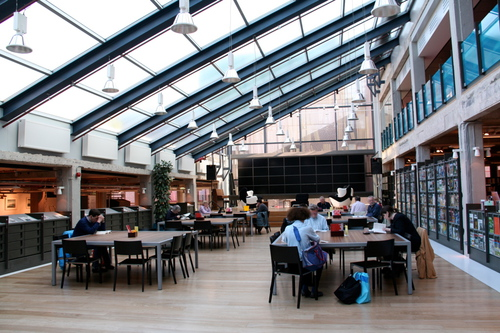
\includegraphics{img/hobohm-3.jpg}
\caption{Abbildung 3: Stadtbibliothek DOK Delft (Bibliothek als dritter
Ort)(2011)}
\end{figure}

Auch für die dritte Komponente im dänischen Modell, die
Beziehungsarbeit, ergeben sich schlagkräftige Beispiele aus Bibliotheken
der letzten Zeit und sei es nur die Dialogkultur der wieder an Bedeutung
gewinnenden sozialen Bibliotheksarbeit oder Aktivitäten wie
\enquote{living libraries} (lebende Bücher) oder der
\enquote{\emph{Heritage Browser}} am Multitouch Table des DOK Delft, an
dem Generationen übergreifende lokale (Familien-) Geschichte
stattfindet. Die Bibliothek als Beziehung (Relation) belässt ihr in
diesem Kontext auch nicht nur eine einfache Differenzqualität zum
Beispiel als Urdefinition von Information, was ja zu der Definition von
Bibliotheken als spezielle Informationssysteme passen würde. Vielmehr
ist hier einerseits suggeriert, dass sich an diesem Ort (auf/in dieser
Arena) Beziehungen (kreativ, selbstständig?) bilden beziehungsweise dass
die ‚Bibliothek` in ihrer Hybridität Beziehungen herstellt. Aus der
dänischen Perspektive bleibt das im Grunde eher politisches Postulat für
die Bibliothek als Motor der Stadtentwicklung. Zahlreiche aktuelle
Beispiele zeigen aber, dass ‚Bibliothek` tatsächlich so funktioniert
oder zumindest auf diese Weise von Architekten, Stadtplanern oder
anderen Stakeholdern der Bibliothek instrumentalisiert wird.

Mit der Setzung der Bibliothek als Ort, Raum und Beziehungskatalysator
ist nun allerdings noch nicht erklärt, warum diese behauptete (neue)
Rollenzuschreibung vor allem auch in ihrer Komplexität funktioniert. Sie
bleibt appellativ oder (be-)wundernd deskriptiv in Fallstudien
gelungener neuer Bibliotheksbauten des Auslands.

Hier gilt es, sich auf andere Grundfunktionen der Bibliothek zu
besinnen. Sie ist ja nicht nur Knoten im Netz der Machtstrukturen und
Werkstatt zur Beförderung von Wissen, sondern immer schon auch konkrete
Instanz für das Funktionsgedächtnis des, wie wir sagen,
\enquote{kulturellen Erbes}. Alle Überlegungen, die Bibliothek nicht
mehr nur als Büchermagazin und Ausleihanstalt zu sehen, versuchen
lediglich, die in der Bücherflut des 19. Jahrhunderts aus dem Blick
geratenen weiteren, nur indirekt thematisierten Funktionen wieder zu
entdecken, ohne wirklich ihre Funktion als Dokumenten- oder
Wissensspeicher tatsächlich in Frage zu stellen. Zu Zeiten des besonders
dringlichen werdenden Problems der Wissensflut entsteht übrigens eine
neue informationswissenschaftliche Subdisziplin: die Dokumentation mit
ihrem verzweifelten Versuch, wenigsten das Wissen der Welt zu
erschließen, wenn man es schon nicht sammeln kann.\footnote{Day, Ronald
  E. (2008): The modern invention of Information. Discourse, history,
  and power. updated and rev. pbk. ed. Carbondale: Southern Illinois
  University Press.}

Die mit den beiden anderen verknüpfte Funktion des Sammelns und
Erschließens des kulturellen Erbes kann besonders anschaulich beobachtet
werden bei dem Dokumentationsunterfangen der Bibliothek des Assurbanipal
zur Bewahrung der eroberten babylonischen Schriften, bei der
Übersetzerwerkstatt der Septuaginta in Alexandria oder selbst bei den
öffentlichen Bibliotheken des römischen Reiches mit ihrem
griechisch-römischen Doppelcharakter. Die Bewahrung des kulturellen
Erbes sorgt sich stets um die Schriftträger und Dokumente der jeweiligen
Zeit sowie um deren Dokumentation, Kulturtransfer und
\emph{re-documentarisation} im neuen Kulturkreis. Oft (wenn nicht immer)
findet dies am Ort und im Raum der Bibliothek statt, zum Beispiel im
Skriptorium. Die aktuellen Bemühungen um \enquote{digitale
Langzeitarchivierung} gehen beispielsweise mit der bibliothekarischen
NESTOR-Initiative in eine ähnliche Richtung wie entsprechende
Bestrebungen zu Zeiten der Renaissance im Zusammenhang mit dem letzten
großen Medienbruch von singulären Papyrus- oder Pergamentrollen zu
seriell produzierten Buch-Kodizes.

Diese Situation näher zu beleuchten versuchte die unter dem Pseudonym
R.T.Pédauque bekannt gewordene (große) französischsprachige
Wissenschaftlergruppe, die die Wiederentdeckung des Dokuments \emph{à la
lumière du numérique} / im Lichte des Digitalen\footnote{Pédauque, Roger
  T. (2006): Le document à la lumière du numérique. Caen: C \& F
  éditions. --- vgl. auch: Pédauque, Roger T. (2007): La
  redocumentarisation du monde. Toulouse: Cépaduès éditions.}
beschreiben half. Schon Ranganathan\footnote{Ranganathan, Shiyali
  Ramamrita (1996): The five laws of library science. Bangalore: Sarada
  Ranganathan Endowment for Library Science (Nachdruck der 2. Aufl. von
  1963). - Buckland, Michael K. (1997): What Is a \enquote{Document}?
  In: Journal of the American Society for Information Science 48 (9), S.
  804--809; S. 807.} hatte das Dokument im Blick als \enquote{embodied
micro thought}, er legte aber den Schwerpunkt auf die durch das Dokument
gegebene synchrone und diachrone Transportmöglichkeit (durch Raum und
Zeit) und die Beständigkeit und Lagerungsfähigkeit von Informationen:

\enquote{{[}a document is an{]} embodied micro thought on paper, or
other material, fit for physical handling, transport across space, and
preservation through time} und: \enquote{record on a more or less flat
surface}.

Die Autorengruppe Pédauque hatte vor dem Hintergrund der zunehmenden
Digitalisierung der Gesellschaft eine funktional-systemische
Beschreibung des Dokuments vorgenommen. Das Dokument funktioniert (nicht
nur im digitalen Zeitalter) in einem dreifachen Spannungsfeld, das
Pédauque mit \enquote{\emph{Vu - Lu - Su}} kennzeichnet: Es muss
überhaupt erst erkennbar sein (\emph{vu}: gesehen), es muss verstanden
und erinnert werden (\emph{lu}: gelesen) und es muss bemerkt und
rezipiert werden (\emph{su}: gewusst). Die Dokument bezogenen
Eigenschaften der Bibliothek beschreibt einer ihrer Autoren, Jean Michel
Salaün, im Kontrast zu den anderen Funktionen und Instanzen des
Dokuments als einen \enquote{immateriell, nicht rivalisierenden} (das
heißt nicht kommerziellen) Aspekt des \enquote{Gedächtnisses} der
\enquote{Gemeinschaft}, bezogen auf die Dokumentdimension
\enquote{\emph{Lu}} -- des Gelesenen.\footnote{Salaün, Jean-Michel
  (2012): Vu, lu, su. Les architectes de l'information face à
  l'oligopole du Web. Paris: la Découverte (Cahiers libres). (eBook)}
Liegt hier eine der Lösungen des zweiten \emph{blind spots} von Wayne
Wiegand?

\newpage
 
 \begin{sidewaystable}
 \footnotesize
 \begin{tabular}{p{0.5cm}p{1.5cm}p{2cm}p{2cm}p{1.5cm}p{2cm}}
 \toprule
 & Funktion & Art & Austausch & Modell & Interface \\
 \cmidrule(r){1-1} \cmidrule(r){2-2} \cmidrule(r){3-3} \cmidrule(r){4-4} \cmidrule(r){5-5} \cmidrule(r){6-6}
 Vu & Kreation & materiell, rivalisierend & Gut, Aneignung & Verlag &
 Autor, Leser\\
 Lu & Gedächtnis & immateriell, nicht-rivalisierend & Zugang,
 Öffentliches Gut & \textbf{Bibliothek} & Gemeinschaft, Leser
 (pl.)\\
 Su & Vermittlung & immateriell, rivalisierend & Aufmerksamkeit,
 Raum-Zeit & Spektakel (Dialog) & Ankündiger, Zuschauer\\
 \cmidrule(r){1-1} \cmidrule(r){2-2} \cmidrule(r){3-3} \cmidrule(r){4-4} \cmidrule(r){5-5} \cmidrule(r){6-6}
 \bottomrule
 \end{tabular}
 \caption{Vu - Lu - Su (nach J.M. Salaün 2012, chap. 4; meine
 +Übertragung)}
 \end{sidewaystable}
 
 \newpage
 

Tabelle 1: Vu - Lu - Su (nach J.M. Salaün 2012, chap. 4; meine
Übertragung)

Bedeutsam bei Pédauque ist jedoch, dass die drei Dimensionen weiterhin
nicht unabhängig von einander stehen, sondern sich bedingen. Salaün
sieht das Dokument nicht unähnlich zu Ranganathan vor allem auch als
Spur zur Vergangenheit, allerdings mit einer konkreten
\enquote{Lektürevereinbarung}, die sich stets aus den anderen
Dimensionen ergibt:

\begin{quote}
\enquote{{[}\ldots{}{]} un document est une trace permettant
d'interpréter un événement passé à partir d'un contrat de
lecture}\footnote{\enquote{\ldots{} ein Dokument ist eine Spur, die
  aufgrund einer Lektürevereinbarung erlaubt, ein vergangenes Ereignis
  zu interpretieren.} (a.a.O.).}
\end{quote}

So ist das Lesen der bibliothekarischen Leser nicht nur von
Alphabetisierung in kultureigener Medientechnik (und Code) abhängig,
sondern steht im Kontext der Spuren der Gemeinschaft in Geschichte und
Gegenwart und erinnert an die französische geschichtswissenschaftliche
Diskussion um die Spuren (traces) von Geschichte\footnote{Vgl. auch:
  Ricoeur, Paul (2009): Archiv, Dokument, Spur. In: Knut Ebeling und
  Stephan Günzel (Hg.): Archivologie. Theorien des Archivs in
  Philosophie, Medien und Künsten. Berlin: Kadmos, S. 123--137.}.

Woher kommt jedoch dieser \emph{contrat de lecture} und wie funktioniert
Lesen sogar als Grundlegung der bibliothekarischen Dokumentensammlung
(und ihrer Rezeption)?

Wieder können wir Michel Foucault bemühen, der sich in seinem Nachwort
\enquote{Un fantastique de bibliothèque}\footnote{Foucault, Michel
  (1979): Un \enquote{fantastique} de bibliothèque. In: Schriften zur
  Literatur. Frankfurt/M u.a.: Ullstein, S. 157--177. (Original 1966)}
zur \emph{Tentation de Saint Antoine} von Flaubert explizit über diese
Dokument-Funktion der Bibliothek ausgelassen hat. Die Bibliothek selbst
ist schuld an so unglücklichen Schicksalen wie dem des Heiligen Antonius
oder des Don Quichotte! Sie ist \enquote{Brutstätte des Geistes} im
positiven Sinn, kann diesen aber auch verwirren (à la Don Quichotte)
oder in Versuchung führen (Saint Antoine). Die Bibliothek ist das
aktivierende Medium und die in ihr angebotene Intertextualität die
Voraussetzung für Gelingen und Scheitern ihrer Akteure, aber auch des
Schreiben, ja der Autorschaft und Leserschaft selbst.

Umberto Eco greift diesen Topos bekanntlich im \emph{Namen der Rose}
wieder auf,\footnote{Taschenbuch-Ausgabe, München: dtv, 1980, S. 366.
  (Hervorhebung von mir)} wenn Adson sinniert:

\begin{quote}
\enquote{Bisher hatte ich immer gedacht, die Bücher sprächen nur von den
menschlichen oder göttlichen Dingen, die sich außerhalb der Bücher
befinden. Nun ging mir plötzlich auf, dass die Bücher nicht selten von
anderen Büchern sprechen, ja, dass es mitunter so ist, als sprächen sie
miteinander. Und im Lichte dieser neuen Erkenntnis erschien mir die
Bibliothek noch unheimlicher. War sie womöglich der Ort eines langen und
säkulären Gewispers, eines unhörbaren Dialogs zwischen Pergament und
Pergament? Also etwas Lebendiges, ein Raum voller \emph{Kräfte, die
durch keinen menschlichen Geist gezähmt werden können}, ein Schatzhaus
voller Geheimnisse, die aus zahllosen Hirnen entsprungen sind und
weiterleben nach dem Tod ihrer Erzeuger? Oder diese fortdauern lassen in
sich?}
\end{quote}

Die Möglichkeit des Schreibens wie des Lesens ist keine (alleinige)
Frage der Kenntnis des Sprach-Systems oder Textkanons, sondern ereignet
sich im \enquote{Raum} der Texte und Diskurse. Schon Ferdinand de
Saussure wies darauf hin, dass nicht die \emph{Langue} (das System/die
Kompetenz) das Wesentliche ist, sondern die \emph{Langage} (also die
Performanz). Jacques Derridas Ansatz der \emph{différance} geht darüber
hinaus und sieht die Semiose als Prozess, der nicht nur linear,
diskursiv und auf das eigene System bezogen ist, sondern ständig
mehrdimensional, den Bezug zum fixen Konzept je verändernd.\footnote{Wem
  dies zu sehr dem überwunden geglaubten Poststrukturalismus entspricht,
  dem sei der aktuelle Beitrag von Hubert Dreyfus und dem
  Kluge-Preisträger Charles Taylor empfohlen, die zugegeben auf
  philosophisch komplexere Weise als Derrida, genau dies den
  \enquote{Ort des Prekonzeptuellen} nennen, der zum Verständnis und zur
  Bewältigung des Realität (und des Seins) notwendig ist. (Dreyfus,
  Hubert L.; Taylor, Charles (2015): Retrieving realism. Cambridge,
  Mass. {[}u.a.{]}: Harvard Univ. Press.)}

Die französische Literaturwissenschaftlerin Julia Kristeva, der das
Verdienst zufällt, den sowjetischen Literaturtheoretiker Michail Bachtin
wiederentdeckt zu haben, betont mit diesem, dass auch die
Intertextualität nicht nur Zitat oder Plagiat des anderen benennbaren
Textes ist, sondern sich im Prozess der Semiose mit ihrem ständigen
Bezug auf den Kontext (vor allem unbewusst und nicht diskursiv)
\emph{ereignet} und so \enquote{latentes narratives Wissen} von
verschiedensten Ursprüngen transportiert.\footnote{Kristeva, Julia
  (1977): Polylogue. Paris: Seuil. -- vgl. Hobohm, Hans-Christoph
  (1991): Der ästhetische Text als Depositum von Weisheit. In: Aleida
  Assmann (Hg.): Weisheit. München: Fink (Archäologie der literarischen
  Kommunikation; III), S. 547--554.} Bachtins eigentliches Thema ist der
\enquote{Chronotopos}, der zunächst als (interne) Zeit- und Ort-bezogene
Erzählstruktur von Geschichten definiert wird, den er aber bei der
Analyse der \enquote{Welt von Rabelais}\footnote{Bachtin, Michail M.
  (1987): Rabelais und seine Welt. Volkskultur als Gegenkultur.
  Frankfurt: Suhrkamp.} auf die gesellschaftliche Narration und den
sozialen Kontext ausweitet. Ort und Zeit sind das Konstituens der
performativen Lektürevereinbarung von Geschichte(n), ob textimanent oder
den Kontext einbeziehend. Nicht von ungefähr ist in vielen Sprachen
\enquote{Geschichte, histoire, storia, history, \ldots{}} das gleiche
Wort wie \enquote{Erzählung, histoire, storia, story, \ldots{}}.

Eine Form von Chronotopologie thematisiert auch der deutsche
Phänomenologe Wilhelm Schapp in seiner Grundlegung des Menschseins als
\enquote{in Geschichten verstrickt}.\footnote{Schapp, Wilhelm (1953): In
  Geschichten verstrickt Zum Sein von Mensch und Ding. Hamburg: Meiner.}
Der Mensch ist als zeitgebundenes Wesen das einzige, das sich der Zeit
bewusst ist. Die menschliche Fähigkeit der Symbolverarbeitung verbindet
sich hier mit seinem Empfinden der Eingebundenheit in Geschichten.
Andere Lebewesen können zwar auch Informationen austauschen, aber nicht
weiterverarbeiten; sie können sich erinnern, aber diese Erinnerungen
nicht \enquote{aufheben} -- schon gar nicht in Geschichte(n). Aber auch
die Sprache ist zeitgebunden und ortsgebunden in der Semiose und in
ihrer Performanz. Der Mensch erlebt sich selbst als Autor und Leser
seiner Geschichte und empfindet sich als sprachliches Wesen als Teil von
anderen Geschichten -- ob gewollt oder ungewollt -- bewusst oder
unbewusst. Er lebt mehr oder weniger bewusst in und zwischen Texten,
Diskursen und Geschichten, die dazu dienen, die Realität zu erfahren, zu
beschreiben und zu interpretieren.

Für den Geschichtsphilosophen Paul Ricoeur, der sich explizit auf Schapp
beruft, ist das die ständige Arbeit an der Mimesis,\footnote{Ricoeur,
  Paul (1983-85): Temps et récit. 3 Bände. Paris: Le Seuil. (dt.:
  \enquote{Zeit und Erzählung}, 3 Bde. München: Fink, 1988-91). -
  Arrien, Sophie-Jan (2007): Ipséité et passivité. Le montage narratif
  du soi (Paul Ricoeur, Wilhelm Schapp et Antonin Artaud). In: Laval
  théologique et philosophique 63 (3), S. 445--458. DOI:
  \href{http://doi.org/10.7202/018171ar}{10.7202/018171ar}.} die nicht
nur die künstlerische Imitation der Realität ist, sondern zum narrativen
Motor der Erzählung des Selbst im ständigen Dialog mit dem \enquote{ich}
wird.\footnote{Ricœur, Paul (2005): Narrative Identität. In: Peter
  Welsen (Hg.): Paul Ricœur: Vom Text zur Person. Hermeneutische
  Aufsätze (1970-1999). Hamburg: Meiner (Philosophische Bibliothek, Bd.
  570), S. 209--226; - Michel, Johann (2003): Narrativité, narration,
  narratologie. du concept ricoeurien d'identité narrative aux sciences
  sociales. In: Revue européenne des sciences sociales 41 (125), S.
  125--142.} Er zieht dabei bewusst beide Aspekte (die Historie und die
Erzählung) zusammen, wenn er deren Funktionieren über die drei
Mimesisstufen: Der \emph{figuration} (\emph{mimesis praxeos:} die
Erfassung der Welt), der \emph{configuration} (der gestalterischen
Arbeit) und der \emph{refiguration} (der Rezeption im weiteren Sinne)
erklärt. Die Arbeit der \emph{figuration} ist nicht bloß Intuition oder
interesse- und konzeptloses Wohlgefallen der Kognition, sondern bedarf
eines \enquote{Gestells} (wie Heidegger sagen würde) oder weiterer
Akteure: Dies sind zum Beispiel die schon vorhandenen Konfigurationen
anderer Geschichten, die Spuren oder vielleicht auch die Dokumente und
Monumente der Historie. Kognition beziehungsweise Erkenntnis ohne diese
ist nicht vorstellbar. Aber auch die Konfiguration der Geschichte
selber, die Mimesis II, wie Ricoeur sie nennt, bedarf der
intertextuellen Einordnung, des Kanons, der Sortierung, Taxonomie oder
der Vitrine (siehe unten).

Erkenntnis (\emph{figuration}) ist stets eine Übersetzung, eine
Vermittlung -- zur \emph{configuration} und damit zunächst Reduktion und
dann aus der Vielfalt der Realität die Verstärkung und Verdeutlichung
der \enquote{figurativen} Elemente durch Standardisierung, Typologie
oder Synopse. Auch wenn dieses Modell bei Ricoeur narratologisch
geschichtsphilosophisch gedacht ist, so zeigt es doch Parallelen zur
vu-lu-su-Trias von Pédauque und damit zum (digitalen) Dokument an sich.
Pédauque hat interessanterweise keine solche chronotopologische
Perspektive. Vielleicht fehlt hier noch die
informationswissenschaftliche Verbindung zum narrativen
Wissensmanagement\footnote{S.oben zum Konzept des \enquote{ba}; sowie:
  Schreyögg, Georg; Koch, Jochen (Hg.) (2005): Knowledge management and
  narratives. Organizational effectiveness through storytelling. Berlin:
  Erich Schmidt.} und die Lösung der Debatte um die Beziehungen zwischen
Dokument, Information und Wissen.\footnote{Hobohm, Hans-Christoph
  (2012): Information und Wissen. In: Konrad Umlauf und Stefan Gradmann
  (Hg.): Handbuch Bibliothek. Geschichte, Aufgaben, Perspektiven.
  Stuttgart: Metzler, S. 73--80.}

Die Beschreibung des menschlichen Erkenntnisprozesses in Bezug auf sein
Verstricktsein in Geschichte(n) und Diskursen ist im Grunde auch die
Resonanz zwischen dem Geschichtsphilosophen Paul Ricoeur und dem
Wissenschaftssoziologen Bruno Latour, denn letztere Argumentation des
Verhältnisses der Erfassung von Welt und ihrer Repräsentation in
Sammlungen stammt aus einem in der Bibliothekswissenschaft leider sehr
wenig beachteten Text\footnote{Latour, Bruno (1996): Ces réseaux que la
  raison ignore - laboratoires, bibliothèques, collections. In:
  Christian Jacob und Marc Baratin (Hg.): Le pouvoir des bibliothèques
  la mémoire des livres en Occident. Paris: Albin Michel (Bibliothèque
  Albin Michel Histoire), S. 23--46.} aus dem Jahre 1996 von Latour
über: \enquote{Diese Netzwerke, die der Verstand nicht wahrnimmt:
Labore, Bibliotheken, Sammlungen}. In einem Band zur politischen
Funktion von Bibliotheken nimmt Latour Stellung zu Bibliotheken, indem
er sie mit seinem Zentralthema, dem wissenschaftlichen Labor und der
wissenschaftlichen Erkenntnistheorie, verbindet. Das Sammeln als Kern
bibliothekarischer Arbeit findet er ebenso bei Naturforschern wie
Alexander von Humboldt, die die Welt in Form der Sammlung von Artefakten
erkunden und diese für eine Erzählung in der Heimat aufbereiten.
Interessanterweise nimmt er seinen Ausgangspunkt ebenso bei der
Intertextualität der Bibliothek, fügt aber an:

\begin{quote}
\enquote{Après quarante années de travaux sur l'intertextualité et le
splendide isolement du monde des signe, il convient de rappeler que les
textes ont prise sur le monde et qu'ils circulent dans les réseaux
pratiques et des institutions qui nous relient à des
situations.}\footnote{Ebd., S. 28: \enquote{Nach vierzig Jahren
  Forschung über Intertextualität und die abgeschiedene Welt der Zeichen
  ist es an der Zeit, daran zu erinnern, dass Texte einen Zugriff auf
  die Welt haben und in praktischen Netzwerken und Institutionen
  zirkulieren, die uns mit Situationen verbinden.} (meine Übertragung)}
\end{quote}

Latour beschreibt die Arbeit des Wissenschaftlers (Autors) zunächst als
Reduktion aus der Fülle der Erkenntnismöglichkeiten. Eine Arbeit, die er
nicht alleine vornimmt, sondern stets geleitet oder unterstützt von
anderen \enquote{Akteuren}, einem Konzept, das die
Akteur-Network-Theorie (ANT) aus der Narratologie von Julien Greimas
entlehnt.\footnote{Greimas, Algirdas Julien (1969): Éléments d'une
  grammaire narrative. In: L'Homme 9 (3), S. 71--92. Online verfügbar
  unter
  \url{http://www.persee.fr/doc/hom_0439-4216_1969_num_9_3_367054}. -
  Greimas, Algirdas Julien (1990): Narrative semiotics and cognitive
  discourses. Aus dem Franz. übers. London: Pinter. - vgl. Ricoeur, Paul
  (1980): La grammaire narrative de Greimas. Documents de recherches
  sémio-linguistique de l'Institut de la langue française, EHESS, CNRS,
  Paris no. 15 (1980).} Solche Akteure können reale Personen sein wie
Assistenten in Natur und Labor, aber auch Erkenntnis leitende Konzepte
oder gar Taxonomien, die zum Beispiel auf Leerstellen hinweisen (auch
dies schon bei Greimas angelegt!). Diese werden schließlich in der
Sammlung der Artefakte des Naturforschers deutlich gemacht durch
Amplifikation, das heißt der Zusammenstellung des Ähnlichen oder
Systematischen, der Synopse der Vitrine (Latour druckt in seinem Text
das Bild einer Vitrine mit ausgestopften Vögeln aus einem
Naturkundemuseum ab) oder eben im Bücherregal. Dem Rezipienten der
Erkenntnis und Sammlungsarbeit des Wissenschaftlers ist gegebenenfalls
eine erneute Reduktion auf das einzelne Objekt vorbehalten, das dieser
aber -- selber wieder als potenzieller Autor -- in die eigene
Amplifikation stellt. Fokussiert man die Arbeit an der \enquote{Natur}
auf den Aspekt einer leitenden Taxonomie, so ist das vor allem die
Arbeit am Kanon des Funktionsgedächtnisses (Assmann) -- die Übersetzung
\enquote{in das Gestell}. Eine diffuse, rein in einer abstrakten Semiose
ablaufende Intertextualität wird geerdet durch die Ausweitung des
Akteurs-Konzepts über den Autor hinaus. Die ANT sieht diesen auch nicht
als bewusst agierenden, sondern eher als Knoten in einem Netz von
Potenzialitäten. In dieser Hinsicht spielt der Ort der Bibliothek als
Werkstatt der Interaktion von Diskursen und Geschichten eben diese Rolle
eines Akteur-Netzwerks. Der Kanon des sagbaren Diskurses, den das
Funktionsgedächtnis ausmacht, muss nicht als normierte Liste oder feste
Struktur verstanden werden, sondern eher als der große gesellschaftliche
Narrativ, von dem Lyotard\footnote{Lyotard, Jean François (1979): La
  condition postmoderne. Rapport sur le savoir. Paris: Minuit.} spricht.
Die \enquote{große Erzählung} ist eine Konfiguration im Sinne Ricoeurs,
die in beiden Richtungen der Mimesis anschlussfähig ist: Als erkenntnis-
und als rezeptionsleitende Instanz. Sie ist aber auch (oder eben gerade
damit) im Sinne Latours ein Akteur, der bei der Reduktion fachlicher
beziehungsweise poetischer Reduktion beiseite steht und \enquote{hilft}.
Die ANT hilft die traditionelle Diskussion um die Mimesis\footnote{Begründer
  des Konzepts und immer noch lesenswert: Auerbach, Erich (1946):
  Mimesis. Dargestellte Wirklichkeit in der abendländischen Literatur.
  Bern: A. Francke.} genauso zu erden wie das ebenso abstrakte Konzept
der Intertextualität.

Konkret bedeutet der Bezug auf die großen Narrative und den Kanon, die
\enquote{Bibliothek als Partner der hegemonialen Instanz} sehen zu
können, zum Beispiel als Bildungseinrichtung, als Ort und Akteur der
sozialen Integration oder auch als informationstechnischer
Innovationsmotor. Bibliotheken haben immer wieder neue Rollen selbst in
Bezug auf die eine hegemoniale Instanz \enquote{Demokratie}.\footnote{Zur
  hegemonialen Instanz: Gramsci, Antonio: \enquote{Hegemony} (1929). In:
  Imre Szeman und Tomithy Kaposy (Hg.) (2011): Cultural theory : an
  anthology. Oxford {[}u.a.{]}: Wiley-Blackwell, S. 188--203.} Der
Konfigurationsprozess ist stets der gleiche, die \enquote{Dokumente}
ändern sich, das \enquote{Gestell} sieht anders aus. Im Zeitalter des
Narrativs \enquote{Innovation und Wachstumsglaube} wird die Public
Library \enquote{Inkubator} und trägt somit genau zu dieser
gemeinschaftlichen figuration/configuration bei, indem sie Makerspaces
betreibt. Hier ist es überdeutlich: Die Bibliothek wird als Akteur
verstanden.

Selbst wenn die Interpretation des Phänomens Bibliothek werkimmanent
bleibt, bekommt sie allein mit dem Konzept der Intertextualität den
Charakter des Mediums, ja des Katalysators. Ihre Erdung mit der ANT und
Ricoeurs (hermeneutischer) Mimesis Konzeption über das Scharnier der
Narratologie und der phänomenologischen Geschichtskonstruktion macht aus
ihr zumindest einen Aktanten im rein narratologischen Sinn von Greimas
oder eben ein Akteur-Netzwerk nach Latour. Das Lesen, die hermeneutische
Refiguration muss an ihrem, an einem Ort stattfinden, betont zumindest
das narrative Wissensmanagement. Aber auch ohne das Konzept des
\enquote{Ba} hier überzustrapazieren, eine konkrete Refiguration ist
ohne Ort (und Zeitpunkt) der Begegnung und des Zusammenwirkens von
Autor, Community und (Massen-) Medien nicht denkbar: Sie funktioniert am
Dokument im Prozess des Vu-Lu-Su.

David Lankes Appell: \enquote{Die Aufgabe der Bibliothekare ist es, die
Gesellschaft zu entwickeln durch die Ermöglichung der Wissensschaffung
in ihren Gemeinschaften}\footnote{\enquote{The Mission of Librarians is
  to Improve Society Through Facilitating Knowledge Creation in Their
  Communities}: Lankes, R. David (2011): The Atlas of New Librarianship.
  Cambridge, Mass: MIT Press; - Lankes, R. David (2012): Expect more.
  Demanding better libraries for today's complex world: Smashwords
  Editions. (dt. Übersetzung in Vorb.)} ist auch in diesem Sinn zu
verstehen. \enquote{Facilitating Knowledge Creation} wird vor allem
durch diesen Prozess der Übersetzung der Realität in gesellschaftliche
Strukturen ermöglicht. Bei Lankes sind dies die \enquote{Konversationen}
von Gordon Pasks \enquote{Conversation Theory}\footnote{Pask, Gordon
  (1976): Conversation theory. Applications in education and
  epistemology. Amsterdam, New York: Elsevier.}, die prekonzeptuelles
Wissen transferieren helfen -- also nicht nur Dokumente im herkömmlichen
Sinn! Es ist Lankes Verdienst, darauf hinzuweisen, dass die Fixierung
der Bibliothekare auf Dokumente im analogen Sinn besonders in einer
digitalen Welt nicht mehr zeitgemäß ist. Von diesem Ausgangspunkt geht
er über Pédauque hinaus und kommt auf einem etwas anderen Weg bei dem
an, was sich ebenso über Foucault, Ricoeur, Latour und schließlich die
dänischen Konzeptionen der Bibliothek (vielleicht europäischer)
begründen lässt: Die Bibliothek als Ort und Akteur der Begegnung von
Geschichten, die Wissen transferieren. 
